% Project de atuação no estágio probatório - 2023-2025
%
%%%%%%%%%%%%%%%%%%%%%%%%%%%%%%%%%%%%%%%%%%%%%%%%%%%%%%%%%%%%%%%%%%%%%%%%%%%%%%%
% Set a class and general configuration
\documentclass[12pt,a4paper,oneside]{book}

%%%%%%%%%%%%%%%%%%%%%%%%%%%%%%%%%%%%%%%%%%%%%%%%%%%%%%%%%%%%%%%%%%%%%%%%%%%%%%%
% Set variables with the title, authors, etc.
\newcommand{\Title}{Projeto de estágio docente}
\newcommand{\Year}{2023}
\newcommand{\Date}{Setembro de \Year{}}
\newcommand{\Author}{Leonardo Uieda}

%%%%%%%%%%%%%%%%%%%%%%%%%%%%%%%%%%%%%%%%%%%%%%%%%%%%%%%%%%%%%%%%%%%%%%%%%%%%%%%
% Import the required packages
\usepackage[utf8]{inputenc}
\usepackage[TU]{fontenc}
\usepackage[brazil]{babel}
\usepackage{amsmath}
\usepackage{amssymb}
\usepackage{graphicx}
\usepackage{hyperref}
\usepackage{fancyhdr}
\usepackage{geometry}
\usepackage{booktabs}
\usepackage{microtype}
\usepackage{siunitx}
\usepackage{xcolor}
% Improved urls with proper hyphenation
\usepackage{xurl}
% Tweak the look of captions
\usepackage{caption}
% To control the style of section titles
\usepackage{titlesec}
% Import natbib and doi packages
\usepackage[round,authoryear,sort]{natbib}
% Add the bibliography to the table of contents
\usepackage[nottoc,chapter]{tocbibind}
% Reference sections by name
\usepackage{nameref}
% Better handling of footnotes inside summary boxes
\usepackage{footmisc}
% Show dois as links on references
\usepackage{doi}
% Remove extra space between references
\usepackage{natbibspacing}
% Use a different font
\usepackage[scaled=0.9,sfdefault]{notomath}
% Icons and fonts (requires using xelatex or luatex)
\usepackage{fontawesome5}
\usepackage{academicons}
% Control the font size
\usepackage{anyfontsize}
\usepackage{setspace}
% To get the number of pages in the document
\usepackage{lastpage}
\usepackage{ragged2e}
% Control over enumerate and itemize
\usepackage{enumitem}
% To define custom environments
\usepackage{environ}
\usepackage{mdframed}
% To control hyphenation for individual blocks of text
\usepackage{hyphenat}
\usepackage{lipsum}

%%%%%%%%%%%%%%%%%%%%%%%%%%%%%%%%%%%%%%%%%%%%%%%%%%%%%%%%%%%%%%%%%%%%%%%%%%%%%%%
% Configuration of the document

\geometry{%
  left=25mm,
  right=25mm,
  top=20mm,
  bottom=15mm,
  headsep=0mm,
  headheight=0mm,
  footskip=5mm,
  includehead=true,
  includefoot=true
}

% Control line and table row spacing
\onehalfspacing
\renewcommand{\arraystretch}{1.5}

% Make urls use the same font as every other text
\urlstyle{same}

% Set the spacing between bibliography entries (requires natbib)
\setlength{\bibsep}{0pt}

% Prevent footnotes from being broken into multiple pages
\interfootnotelinepenalty=10000

% Customize how Chapter headings are displayed
\titleclass{\chapter}{straight}
\titleformat{\chapter}[display]{\normalfont}{}{0pt}{\onehalfspacing\ifnum\thechapter>0 \Large\thechapter. \fi\huge}[\titlerule]
\titlespacing*{\chapter}{0pt}{10pt}{20pt}

% Custom colors
\definecolor{darkgray}{gray}{0.4}
\definecolor{mediumgray}{gray}{0.5}
\definecolor{lightgray}{gray}{0.9}
\definecolor{mediumblue}{HTML}{2060c2}
\definecolor{lightblue}{HTML}{f7faff}

% Configure captions
\captionsetup[table]{position=below,skip=0pt}
\captionsetup{labelfont=bf,font={small,color=darkgray},skip=10pt}

% Configure hyperref and add PDF metadata
\hypersetup{
    colorlinks,
    allcolors=mediumblue,
    pdftitle={\Title},
    pdfauthor={\Author},
    breaklinks=true,
}

% Configure header and footer
% Inspired by LaPreprint: https://github.com/roaldarbol/LaPreprint
\renewcommand{\chaptermark}[1]{\markboth{#1}{}}
\newcommand{\Separator}{\hspace{3pt}|\hspace{3pt}}
\newcommand{\FooterFont}{\footnotesize\color{mediumgray}}
\pagestyle{fancy}
\fancyhf{}
\lfoot{%
  \FooterFont{}
  \leftmark{}
}
\rfoot{%
  \FooterFont{}
  \thepage\space de\space \pageref*{LastPage}
}
\renewcommand{\headrulewidth}{0pt}
\renewcommand{\footrulewidth}{1pt}
\preto{\footrule}{\color{lightgray}}
\fancypagestyle{plain}{%
  \fancyhf{}
  \cfoot{%
    \FooterFont{}
    \Title{}
    \Separator{}
    \Author{}
  }
}

% Define fancy text boxes
\NewEnviron{summarybox}[1]{%
  \mdfdefinestyle{summarybox_}{%
    leftline=true,
    rightline=false,
    topline=false,
    bottomline=false,
    linewidth=3pt,
    linecolor=mediumblue,
    backgroundcolor=lightblue,
    innertopmargin=12pt,
    innerbottommargin=12pt,
    innerleftmargin=12pt,
    innerrightmargin=12pt,
    skipbelow=15pt,
    skipabove=15pt,
    frametitleaboveskip=12pt,
    frametitlebelowskip=5pt,
  }
  \newmdenv[style=summarybox_]{summarybox_}
  \begin{summarybox_}[frametitle=#1]
    \BODY
  \end{summarybox_}
}

% Make a list with no margin and smaller spacing for use with the summaryboxes
\NewEnviron{listnomargin}[1]{%
  % Remove spacing between enumerate/itemize items
  \setlist{nosep}
  \begin{#1}[leftmargin=*]
    \BODY
  \end{#1}
}

%%%%%%%%%%%%%%%%%%%%%%%%%%%%%%%%%%%%%%%%%%%%%%%%%%%%%%%%%%%%%%%%%%%%%%%%%%%%%%%
\begin{document}

\pagestyle{empty}
\frontmatter

\begin{titlepage}
  \begin{center}
    
\includegraphics[height=1.5cm]{figures/usp.png}
    \hfill
    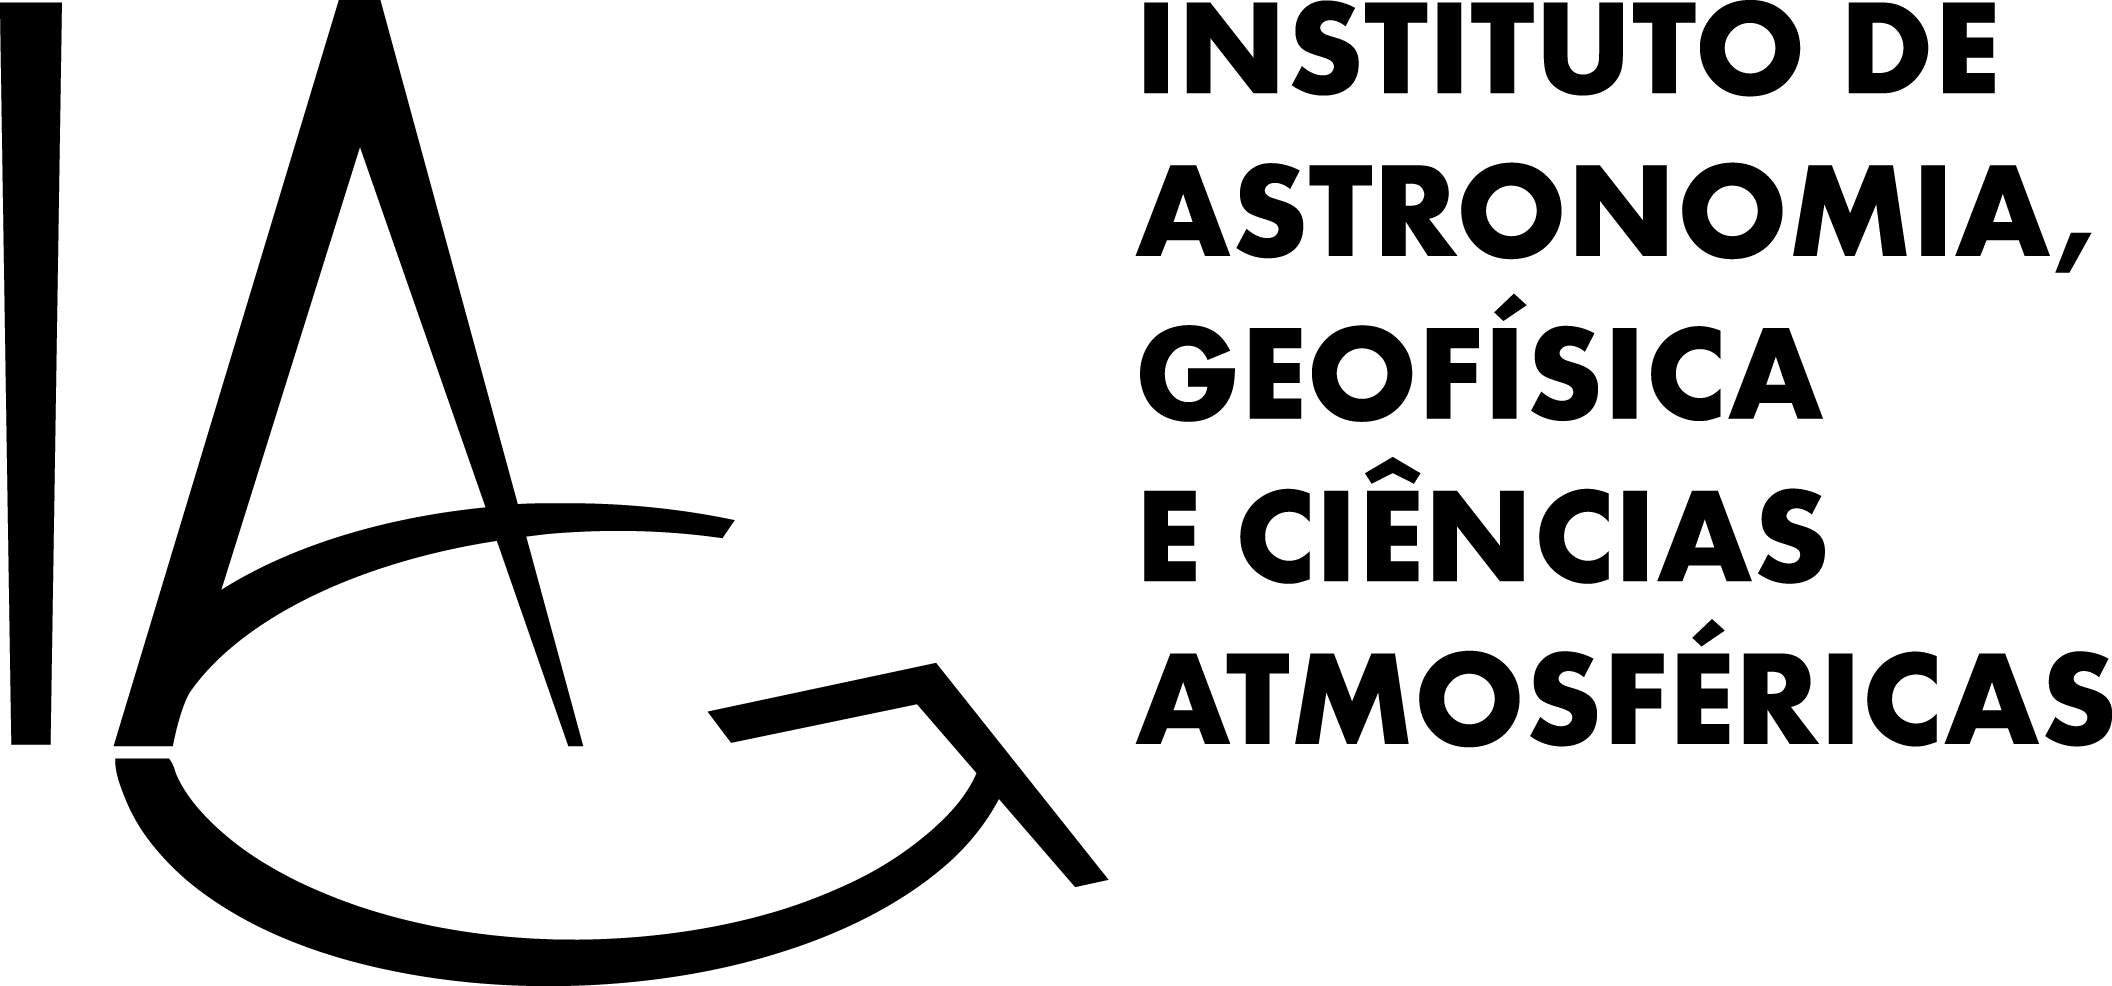
\includegraphics[height=1.5cm]{figures/iag.png}
    \vspace{9cm}

    \textbf{\Huge \MakeUppercase{\Title{}}}
    \vspace{2cm}

    \textbf{\LARGE \Author{}}
    \vfill

    Departamento de Geofísica
    \\
    Instituto de Astronomia, Geofísica e Ciências Atmosféricas
    \\
    Universidade de São Paulo
    \vspace{2cm}

    \Date{}
  \end{center}
\end{titlepage}

\tableofcontents

\mainmatter
\pagestyle{fancy}

%==============================================================================
\chapter{Introdução}

Este projeto apresenta meu plano de atuação como Professor Doutor do
Departamento de Geofísica do Instituto de Astronomia, Geofísica e Ciências
Atmosféricas da Universidade de São Paulo para os próximos dois anos, entre
setembro de 2023 e agosto de 2025.
O plano de atividades abrange as áreas de ensino, extensão, pesquisa e gestão
universitária.
Um fator que é comum a todas essas áreas é minha dedicação ao uso e ao
desenvolvimento de ferramentas abertas e gratuitas para comunidade, incluindo
software livre e recursos educacionais
abertos\footnote{\url{https://www.unesco.org/en/open-educational-resources}}.


%==============================================================================
\chapter{Extensão e cultura}

Minha experiência prévia na área de extensão inclui a produção de vídeos,
cursos de curta duração, voluntariado em escolas e participação nas feiras de
profissões da Universidade de Liverpool.
Meus planos de atuação nesta área para os próximos dois anos são:

\begin{enumerate}
  \item \textbf{Escola de Verão da Geofísica:} O Departamento de Geofísica
    organiza anualmente uma Escola de Verão com cursos de curta duração em
    diversas áreas. Estes cursos são oferecidos tanto para alunos da
    instituição quanto para a comunidade externa. Os cursos proporcionam uma
    oportunidade de inserir temas atuais e relevantes na grade curricular,
    ministrados por especialistas internos e externos à USP. Ministrei dois
    cursos na Escola de Verão em 2012 e 2016. Pretendo propor novos cursos em
    edições futuras, possivelmente nas áreas de problemas inversos,
    processamento de dados de métodos potenciais, aprendizagem de máquinas e
    desenvolvimento de software livre.
  \item \textbf{Feira USP e as Profissões:} A feira é organizada anualmente
    pela universidade e tem como objetivo a divulgação dos cursos e recursos da
    USP para vestibulandos e demais interessados. Estas atividades são cruciais
    para a divulgação do curso de Bacharelado em Geofísica, que é pouco conhecido
    pela comunidade (como indicado no Plano Acadêmico Departamental 2018-2022).
    Pretendo participar da Feira e futuramente propor atividades que poderiam
    ser executadas durante edições futuras.
  \item \textbf{Curso de Palhaçaria Científica:} Estou participando como
    colaborador do projeto ``Palhaçaria Científica'', coordenado pelo Prof.
    George Sand Leão Araújo de França. O curso tem como objetivo treinar
    cientistas (alunos, docentes e posdocs) e professores de ciências no uso da
    palhaçaria para divulgação de conceitos científicos de maneira descontraída
    e criativa. Minhas contribuições serão na parte de organização e divulgação
    do curso. Um projeto inicial foi submetido à Pró-Reitoria de Cultura e
    Extensão Universitária para o financiamento de um curso em 2024, no qual
    pretendo participar também como aluno. Caso seja bem sucedido, pretendemos
    expandir o curso e pleitear recursos externos para futuras edições.
  \item \textbf{SEG Student Chapter:} A Society of Exploration Geophysicists
    (SEG) possui um programa de ``capítulos estudantis'' com abrangência
    mundial. Os capítulos são formados por alunos de programas de graduação e
    pós-graduação de cursos de geofísica e áreas afins. Os capítulos
    representam a unidade junto á SEG e recebem recursos e vantagens em troca
    da divulgação da sociedade eme suas unidades. Os benefícios incluem:
    participação no congresso anual da SEG nos Estados Unidos; visita de
    palestrantes internacionais; participação na competição SEG Challenge Bowl;
    participação em eventos de treinamento; doação de livros técnicos. Durante
    minha estadia na UERJ, auxiliei os alunos do curso de Geologia na criação
    de um capítulo da SEG. Esta atividade foi muito proveitosa para os alunos
    e gerou um aumento grande no interesse dos alunos pela geofísica. Pretendo
    iniciar um diálogo com os alunos de graduação e pós-graduação do IAG para
    incentivar a retomada das atividades do capítulo (atividade destacada no
    Plano Departamental). Pretendo também auxiliar na organização da estrutura
    administrativa do capítulo e na divulgação de suas atividades.
  \item \textbf{Organização de um \emph{workshop} sobre software livre na
    geofísica:}
    As comunidades de software livre Fatiando a
    Terra\footnote{\url{https://www.fatiando.org}} (criado e liderado por mim)
    e SimPEG\footnote{\url{https://simpeg.xyz/}}
    (criado pelo grupo de inversão da University of British Columbia),
    desenvolvem software livre em linguagem Python para modelagem e
    processamento de dados geofísicos a mais de uma década. Ambos contam com uma
    gama de voluntários que desenvolvem o código, organizam eventos, escrevem
    documentação e dão apoio a novos usuários e desenvolvedores.
    Em julho de 2023, realizamos o primeiro workshop conjunto das duas
    comunidades, intitulado
    ``Open-Source Tools to Enable Geophysical Data Processing and
    Inversion\footnote{\url{https://birs-2023.softwareunderground.org/}}'', na
    Banff International Resarch Station (BIRS). Os objetivos do workshop eram
    promover a colaboração entre os dois projetos e aumentar a conexão entre os
    desenvolvedores dos projetos e seus usuários, tanto na pesquisa acadêmica
    quanto no setor privado. Pretendo dar início à organização de um workshop
    subsequente, realizado no estado de São Paulo, para dar continuidade aos
    trabalhos iniciados na BIRS e para conectar a comunidade geofísica
    brasileira com os dois projetos (por exemplo, incluindo geocientistas do
    Serviço Geológico do Brasil (CPRM), da Vale, do IAG, do Observatório
    Nacional, etc.). Planejo pleitear por auxílio financeiro da FAPESP e de
    parceiros nos setores privado e público para a organização do evento, que
    poderá ser executado em 2025.
\end{enumerate}


%==============================================================================
\chapter{Funções de gestão universitária}

Durante esses primeiros dois anos na USP, planejo iniciar atividades de gestão
universitária de forma gradativa, acumulado responsabilidades e experiência.
Inicialmente, gostaria de participar das seguintes comissões:

\begin{enumerate}
  \item \textbf{Comissão de Cooperação Nacional e Internacional:} Acredito que
    possa fazer contribuições relevantes aos trabalhos dessa comissão através
    de minha experiência internacional nos Estados Unidos, Canadá e Reino
    Unido.
  \item \textbf{Comissão Coordenadora de Curso - Bacharelado em Geofísica:}
    Possuo experiência prévia na coordenação do curso de Bacharelado em
    Geofísica da Universidade de Liverpool, podendo trazer uma perspectiva
    internacional para a reforma da grade curricular que está sendo planejada.
    Por exemplo, os cursos de Liverpool implementavam um sistema de tutoria e
    ciclo básico único com especializações, ambas mudanças planejadas para os
    cursos do IAG (conforme indicado no Plano Acadêmico Departamental).
\end{enumerate}



%==============================================================================
\chapter{Atividade didática}

Possuo experiência prévia em sala de aula a nível de graduação, em cursos de
curta duração (presenciais e online), ensino a distância (durante a pandemia de
COVID-19), na produção de recursos educacionais abertos e na orientação de
alunos de graduação, mestrado e doutorado.
Nos próximos dois anos, pretendo continuar com atividades em todas essas
frentes e expandir meu grupo de pesquisa através da orientação de alunos de
IC e pós-graduação.

\section{Disciplinas}

Inicialmente, ministrarei as disciplinas:

\begin{enumerate}
  \item \textbf{AGG0011 - Problemas Integrados em Ciências da Terra I:}
    Disciplina obrigatória do 2º período do curso de Bacharelado em Geofísica do IAG.
    Dividida com os Profs. Eder Cassola Molina e Marcelo Belentani de
    Bianchi.
  \item \textbf{AGG0110 - Elementos de Geofísica:}
    Disciplina obrigatória do curso de Licenciatura em Geociências do IGc.
    Dividida com a Prof. Daniele Cornellio de Paiva Caldeira Brandt e o Prof.
    Marcelo Belentani de Bianchi.
  \item \textbf{AGG0204 - Computação para Geofísicos:}
    Disciplina optativa do curso de Bacharelado em Geofísica do IAG.
    Dividida com o Prof. Victor Sacek.
  \item \textbf{AGG0669 - Gravimetria e Magnetometria Aplicadas à Prospecção de
    Bens Minerais e Estruturas Crustais:}
    Disciplina obrigatória do 8º período do curso de Bacharelado em Geofísica do IAG.
    Dividida com o Prof. Eder Cassola Molina.
  \item \textbf{AGG5740 - Teoria de Inversão em Geofísica:}
    Disciplina optativa pós-graduação em Geofísica do IAG.
    Assumirei essa disciplina em 2024 ou 2025, dependendo da disponibilidade
    do Prof. Carlos Alberto Moreno Chaves, atual responsável por ela.
\end{enumerate}

No futuro próximo também pretendo avaliar a possibilidade da criação de uma
disciplina optativa na área de métodos potenciais. Esta disciplina se
encaixaria no último ano da graduação em geofísica e possuiria uma disciplina
equivalente no programa de pós-graduação que seria ofertada simultaneamente com
a da graduação. O objetivo seria cobrir a falta de uma disciplina específica de
métodos potenciais na pós-graduação e oferecer aos alunos da graduação uma
oportunidade de aprofundar seus conhecimentos do assunto.
O foco da disciplina será na interpretação e modelagem de dados reais, tanto em
escala global (através de modelos geopotenciais) quanto em escala regional e
local (através de conjuntos de dados abertos).



\section{Produção de recursos educacionais abertos}

Os recursos educacionais abertos que pretendo produzir se encaixam em duas
categorias principais:

\begin{enumerate}
  \item \textbf{Material didático para uma disciplina específica:} O material
    que criarei e adaptarei para as disciplinas listadas acima será
    disponibilizado em formato digital na plataforma GitHub\footnote{Por exemplo,
    \url{https://github.com/leouieda/geofisica1}.} sob uma licença aberta (CC-BY
    e MIT). Este material é destinado a ser utilizado nas disciplinas
    específicas mas tem potencial para ser reaproveitado e modificado em outros
    cursos através da licença adotada.
  \item \textbf{Livros e apostilas em formato digital:}
    Ao adquirir experiência nas disciplinas listadas na sessão anterior,
    buscarei identificar onde existem lacunas ainda não cobertas por livros
    texto, que necessitem de atualização, ou cujo livro texto é inacessível a
    determinados alunos (pelo custo monetário, nível de conhecimento, língua,
    etc.). Uma vez identificadas estas lacunas, pretendo desenvolver livros e
    apostilas em formato digital (com a ferramenta
    JupyterBook\footnote{\url{https://jupyterbook.org}}) que serão
    disponibilizados gratuitamente na plataforma GitHub dentro da organização
    Geophysics Library\footnote{\url{https://github.com/GeophysicsLibrary/}}.
    Este material didático servirá como apoio ao material específico das
    disciplinas. Seu desenvolvimento se dará de forma gradativa e buscarei
    colaboradores nacionais e internacionais para seu desenvolvimento.
    O desenvolvimento deste material também poderá ser efetuado com
    participação de alunos através de bolsas do Programa Unificado de Bolsas de
    Estudos para apoio à Formação de Estudantes de Graduação da USP. Nos
    próximos dois anos, meu objetivo principal é identificar as áreas nas quais
    devo investir mais tempo e iniciar o contato com possíveis colaboradores.
\end{enumerate}


\section{Orientação de estudantes}

Atualmente, estou orientando dois alunos de doutorado:

\begin{enumerate}
  \item \textbf{India Uppal:} Aluna de doutorado da Universidade de Liverpool.
    Fui seu orientador até agosto de 2023, quando saí da Universidade de
    Liverpool. Atualmente sou seu coorientador e seu orientador é o Prof.
    Richard Holme. India está começando seu terceiro ano de doutorado (o prazo
    para a conclusão do doutorado é de seis anos).
  \item \textbf{Gelson Ferreira de Souza Junior:} Aluno de doutorado em
    geofísica do IAG. Sou coorientador do Gelson e seu orientador é o Prof.
    Ricardo Ivan Ferreira da Trindade. Em setembro de 2023, entramos com o
    pedido de transferência de orientação para mim. Gelson também está no
    início de seu terceiro ano de doutorado com bolsa da FAPESP.
\end{enumerate}

Como parte das atividades de pesquisa discutidas no próximo capítulo, pretendo
recrutar alunos de iniciação científica e pós-graduação nas seguintes áreas:

\begin{enumerate}
  \item \textbf{Desenvolvimento de software livre para geofísica (1 ou 2 vagas
    para iniciação científica):} O projeto envolve a implementação em linguagem
    Python de métodos para processamento e modelagem de dados gravimétricos e
    magnetométricos. Estudantes envolvidos serão treinados em técnicas de
    engenharia de software (controle de versão, testes unitários, documentação)
    e o código será integrado diretamente no software
    Harmonica\footnote{\url{https://github.com/fatiando/harmonica}}.
    Este projeto fornecerá aos alunos experiência prática em pesquisa
    metodológica, desenvolvimento de software a nível profissional, ciência de
    dados e metodologias de ponto na geofísica.
  \item \textbf{Integração de dados gravimétricos utilizando fontes
    equivalentes (mestrado):}
    O projeto tem como objetivo investigar o uso da técnicas de fontes
    equivalentes desenvolvida em \citet{Soler2021} para a integração de dados
    gravimétricos terrestres, aéreos e de satélite. A técnica será testada no
    conjunto de dados gravimétricos australiano, que disponibiliza milhares de
    pontos de observação com uma licença de dados abertos. Os resultados
    esperados são avanços metodológicos em fontes equivalentes e a geração de
    uma nova malha regular de dados para a Austrália que inclui toda a gama de
    observações disponíveis. Estes resultados poderão ser implementados no
    Brasil caso um conjunto de dados semelhantes seja disponibilizado
    abertamente.
  \item \textbf{Inversão 3D de dados magnéticos para determinação da isoterma
    de Curie em coordenadas esféricas (doutorado):}
    Este projeto irá adaptar o método de \citet{Uieda2017} para a inversão de
    dados de amplitude do campo magnético anômalo que serão produzidos pela
    aluna India Uppal para a Antártica. O desenvolvimento do método terá
    diversos desafios, como o grande volume de dados, a implementação de
    vínculos para a estimativa da susceptibilidade magnética e a instabilidade
    da modelagem direta em torno do polo geográfico. A isoterma de Curie gerada
    neste projeto poderá ser convertida em estimativa do fluxo geotermal
    subglacial e utilizada na interpretação da evolução tectônica da Antártica.
\end{enumerate}

A orientação de alunos abrange mais do que o projeto de pesquisa. Acredito que
seja necessário fornecer treinamentos que se alinhem com os objetivos de
carreira de cada aluno, seja na pesquisa acadêmica, na indústria ou no ensino.


Colocar parte de formação extra-curricular e preparo para o mercado de trabalho
fora do setor acadêmico.



%==============================================================================
\chapter{Pesquisa}

Nos últimos anos, tenho priorizado as seguintes linhas de pesquisa:

\begin{enumerate}
  \item \textbf{Integração de dados gravimétricos e magnetométricos:}
    Dados dos campos de gravidade e magnético são adquiridos em escala local,
    regional (aerolevantamentos) e global (satélites). A integração destes
    diferentes conjuntos de dados para a produção de uma malha regular a
    altitude constante gera desafios computacionais (devido a quantidade de dados) e metodológicos (devido à disparidade de cobertura, acurácia e altitudes
    de aquisição). Nesta linha, busco desenvolver métodos que permitam superar
    esses desafios. Meu foco tem sido na combinação da técnica de fontes
    equivalentes com métodos de aprendizagem de máquinas.
  \item \textbf{Problemas inversos em 3D:}
\end{enumerate}

linha de pesquisa, em Geofísica, três projetos de pesquisa e um de ensino e
extensão: Projeto 1: Geodinâmica; Projeto 2: Geofísica Aplicada; Projeto 3: Modelagem e
Ciência de Dados em Geofísica


\section{%
  Projeto 1: Integração de dados magnéticos aéreos e de satélite sobre o
  continente Antártico
}

\subsection{Enunciado do problema}
% Qual será o problema tratado pelo projeto e qual sua importância? Qual será a
% contribuição para a área se bem-sucedido? Cite trabalhos relevantes na área,
% conforme necessário.

O fluxo geotermal, que é a taxa de variação vertical de calor vindo da
crosta terrestre, é considerado um importante fator que influencia a evolução
das geleiras na Antártica \citep{Seroussi2017}.
Um grande esforço tem sido feito recentemente pela comunidade científica para
melhor entender a variação espacial do fluxo geotermal antártico e seu papel
durante esse período de mudanças climáticas \citep{BurtonJohnson2020}.
Porém, o fluxo geotermal nas regiões polares ainda é pouco conhecido devido à
dificuldade de se obter medições diretas desse parâmetro no ambiente hostil no
interior do continente antártico \citep{BurtonJohnson2020}.
Com a escassez de medições diretas, se torna necessário estimar o fluxo
geotermal na base das geleiras utilizando a geofísica, como a tomografia
sísmica, a magnetometria e a gravimetria.
Dados magnéticos são frequentemente usados, tanto provenientes de aquisições
aéreas \citep[e.g.,][]{Lowe2023} quanto de satélites
\citep[e.g.,][]{FoxMaule2005}.

A relação entre as anomalias magnéticas provindas da litosfera terrestre e o
fluxo geotermal na superfície é indireta e depende de diversas premissas.
Assumindo que a magnetização da crosta se dá numa direção próxima à do campo
geomagnético (i.e., a magnetização é predominantemente induzida), é possível
estimar a profundidade máxima das fontes magnéticas \citep{Spector1970}.
Essa profundidade nos informa onde as rochas atingem a temperatura de Curie,
na qual os minerais ferromagnéticos perdem sua capacidade de armazenar
magnetização e se tornam paramagnéticos com uma baixa susceptibilidade
magnética \citep{Blakely1988}.
Se as fontes magnéticas forem compostas do mineral magnetita, podemos então
deduzir que uma isoterma de aproximadamente \qty{580}{\degreeCelsius} (a
temperatura de Curie da magnetita) se encontra na profundidade estimada.
Sabendo a temperatura em profundidade e na superfície, podemos finalmente
estimar o fluxo geotermal na superfície $q_z$ utilizando uma aproximação para a
Lei de Fourier

\begin{equation}
  q_z = c_t \dfrac{\partial T}{\partial z} \approx c_t \dfrac{T_s - T_c}{\Delta z_c},
\end{equation}

\noindent
onde $c_t$ é a condutividade térmica das rochas, $T$ é a temperatura, $z$ é a
coordenada vertical, $\Delta z_c$ é a profundidade da isoterma de Curie (obtida
através dos dados magnéticos) e $T_s$ e $T_c$ são a temperatura na superfície e
a temperatura de Curie, respectivamente.
Nesta equação se encontra a última premissa deste processo: assume-se que a
condutividade térmica das rochas é uniforme e que seu valor é conhecido.

A classe de métodos mais popular para se obter a profundidade da isoterma de
Curie a partir de dados magnéticos utiliza uma relação estatística entre o
espectro de amplitudes dos dados e a profundidade das fontes magnéticas
\citep{BurtonJohnson2020}.
Essa relação foi estabelecida por \citet{Spector1970} para obter uma
profundidade média do topo e da base do conjunto de fontes magnéticas em uma
área.
Desde então, o método foi aprimorado por diversos autores \citep[uma revisão
dos métodos e suas limitações pode ser encontrada em ][]{NunezDemarco2020}.
Para obter uma distribuição espacial das profundidades, alguns trabalhos
dividem a área de investigação em janelas com uma certa sobreposição e estimam
a profundidade das fontes dentro de cada janela.
Os métodos derivados de \citet{Spector1970} se tornaram ubíquos devido a sua
simplicidade e eficiência computacional.
Porém, existem críticas do uso indiscriminado do método
\citep{Johnson2016,NunezDemarco2020}.
Por exemplo, \citet{Johnson2016} recomendam seu uso somente como uma estimativa
inicial das características gerais da área de investigação antes de se utilizar
métodos mais sofisticados de modelagem direta e inversa.

Não é difícil prever que a incerteza das estimativas de fluxo geotermal a
partir de dados magnéticos será grande, envolvendo erros na compilação dos
dados aeromagnéticos e também as limitações do método em si
\citep{BurtonJohnson2020}.
Estudos recentes utilizando dados magnéticos para aprendizagem de máquinas
\citep{Losing2021} e para reconstruções paleogeográficas \citep{Ebbing2021} tem
apresentado resultados promissores.
\citet{Ebbing2021} sugerem que a integração de dados de satélite e
aeromagnéticos é necessária, enquanto \citet{Lowe2023} argumentam que a alta
resolução dos dados de aerolevantamentos devem ser preservadas.
Os dados magnéticos também são utilizados para treinar os algoritmos de
aprendizagem de máquinas.
Logo, esses dados necessitam ser de alta qualidade para obter previsões
confiáveis.

Considerando os pontos descritas acima, fica claro que é essencial obter novas
formas de:

\begin{enumerate}
  \item Integrar dados de satélite e aerolevantamentos para providenciar uma
    cobertura total do continente e, ao mesmo tempo, preservar a alta resolução
    dos dados aeromagnéticos.
  \item Transformar dados da anomalia magnética do campo total em quantidades
    que sejam menos sensíveis à direção de magnetização das fontes, como a
    amplitude do campo magnético anômalo \citep{Melo2021}. Lembrando que os
    métodos para obter a profundidade da isoterma de Curie assumem conhecimento
    sobre a direção de magnetização das fontes.
  \item Estimar a profundidade da isoterma de Curie a partir de dados
    magnéticos utilizando métodos mais sofisticados de inversão,
    preferencialmente em uma aproximação esférica da Terra devido ao tamanho da
    Antártica.
\end{enumerate}

% Qual será o problema tratado pelo projeto e qual sua importância? Qual será a
% contribuição para a área se bem-sucedido? Cite trabalhos relevantes na área,
% conforme necessário.
\noindent
Neste projeto, iremos desenvolver métodos numéricos e ferramentas
computacionais abertas para resolver essas questões.
As soluções encontradas poderão levar a novos entendimentos sobre a estrutura
crustal e evolução tectônica da Antártica, sobre as limitações do uso de dados
magnéticos mesmo com métodos novos de processamento e também sobre os fatores
que controlam o fluxo geotermal embaixo das geleiras.

\begin{summarybox}{\faBullseye{} Objetivos principais}
  \begin{listnomargin}{enumerate}
    \item Combinar todos os dados magnéticos de satélite e aéreos disponíveis
      para a Antártica em um novo conjunto de dados com espaçamento e altitude
      uniformes.
    \item Transformar os dados de anomalia magnética de campo total ($\Delta
      T$) em dados de amplitude total do campo magnético anômalo
      ($\|\mathbf{B}\|$), que são menos sensíveis à variações na direção de
      magnetização das fontes.
    \item Utilizar os novos dados de amplitude total do campo para estimar a
      profundidade da isoterma de Curie e o fluxo geotermal na base das
      geleiras antárticas.
  \end{listnomargin}
\end{summarybox}

\subsection{Resultados esperados}
% O que será criado ou produzido como resultado o projeto proposto?

Este projeto está divido em três epatas:

\begin{itemize}
  \item \textbf{Etapa 1:} Integração de dados magnéticos utilizando fontes
    equivalentes.
  \item \textbf{Etapa 2:} Transformação de dados de anomalia magnética de campo
    total em dados de amplitude do campo magnético anômalo utilizando fontes
    equivalentes.
  \item \textbf{Etapa 3:} Estimativa da profundidade da isoterma de Curie
    utilizando um método de inversão não-linear em uma aproximação esférica.
\end{itemize}

\noindent
Esperamos que este projeto produza os seguintes resultados:

\begin{enumerate}
  \item Uma nova maneira de integrar dados magnéticos de satélite e de
    levantamentos aerogeofísicos utilizando o método de
    \textit{gradient-boosted equivalent sources} \citep{Soler2021} com uma
    resolução nunca antes alcançada [etapa 1].
  \item Conhecimento proveniente de resultados experimentais sobre as vantagens
    e limitações do uso da \textit{amplitude do campo magnético anômalo} no
    contexto antártico para a interpretação geológica \citep{Melo2021} e a
    recuperação da profundidade da isoterma de Curie \citep{HidalgoGato2021}
    [etapas 2 e 3].
  \item Um novo método de inversão, baseado em \citet{Uieda2017} e
    \citet{HidalgoGato2021}, para estimar a profundidade da isoterma de Curie
    em uma aproximação esférica da Terra a partir de dados da amplitude do
    campo magnético anômalo e com vínculos provenientes de outros dados
    geofísicos [etapa 3].
  \item Uma nova estimativa da isoterma de Curie e do fluxo geotermal com maior
    resolução espacial e consistência com outras estimativas [etapa 3].
\end{enumerate}

\noindent
Além disso, o projeto também poderá gerar os seguintes recursos para a
comunidade científica, todos disponibilizados gratuitamente sob licenças
abertas:

\begin{enumerate}
  \item Componentes adicionadas ao software livre Harmonica para:
    1) a combinação de dados magnéticos e a sua transformação em dados de
       amplitude do campo anômalo utilizando fontes equivalentes [etapas 1 e
       2];
    2) a inversão dos dados magnéticos em coordenadas esféricas para estimar a
       profundidade da isoterma de Curie [etapa 3].
  \item Uma nova compilação de dados magnéticos para a Antártica na forma de
    uma malha regular com altitude controlada cobrindo todo o continente e os
    oceanos adjacentes [etapas 1 e 2].
\end{enumerate}

\subsection{Disseminação e avaliação}
% Como os resultados do projeto deverão ser avaliados e como serão
% disseminados?

Os resultados provenientes deste projeto serão avaliados utilizando:

\begin{itemize}
  \item Testes com dados sintéticos utilizando modelos geologicamente
    plausíveis. Nestes testes, sabemos qual é o resultado esperado e então
    podemos calcular o erro cometido pelos métodos desenvolvidos. Através de
    dados sintéticos, podemos também avaliar as limitações dos métodos e ganhar
    experiência para diagnosticar problemas que podem ocorrer na aplicação a
    dados reais.
  \item Comparação com resultados anteriores. Por exemplo, as compilações de
    dados magnéticos ADMAP-2 e ADMAP-2s \citep{Golynsky2018, Kim2022} e outros
    modelos de fluxo geotermal \citep{FoxMaule2005, Losing2021, Losing2020,
    Stal2021}.
\end{itemize}

\noindent
A disseminação dos resultados será feita através de:

\begin{itemize}
  \item Artigos em periódicos internacionais.
  \item Campanhas em mídias sociais no formato de e-pôsteres.
  \item Apresentação dos resultados em congressos internacionais da EGU, AGU e
    SCAR.
  \item Tutoriais em formato de páginas na internet e vídeos que explicam como
    utilizar os métodos desenvolvidos para outras aplicações.
  \item Vídeos de divulgação científica para o público geral. Criadores com
    audiência estabelecida na plataforma YouTube (por exemplo,
    \href{https://www.youtube.com/@MinuteEarth}{MinuteEarth} ou
    \href{https://www.youtube.com/@manualdomundo}{Manual do Mundo})
    serão contratados para produzir os vídeos\footnote{Um exemplo disso é este
    vídeo, que tem mais de meio de milhão de visualizações, feito pelo canal
    MinuteEarth para divulgar os resultados de um projeto da NSF:
    \url{https://youtu.be/J6d0UqY6IsA}}.
\end{itemize}

%==============================================================================
\backmatter
\bibliographystyle{apalike-doi}
\bibliography{references}
\chaptermark{Referências Bibliográficas}

\end{document}
